\begin{minipage}{0.55\textwidth}
    \begin{figure}[h]
    \centering
    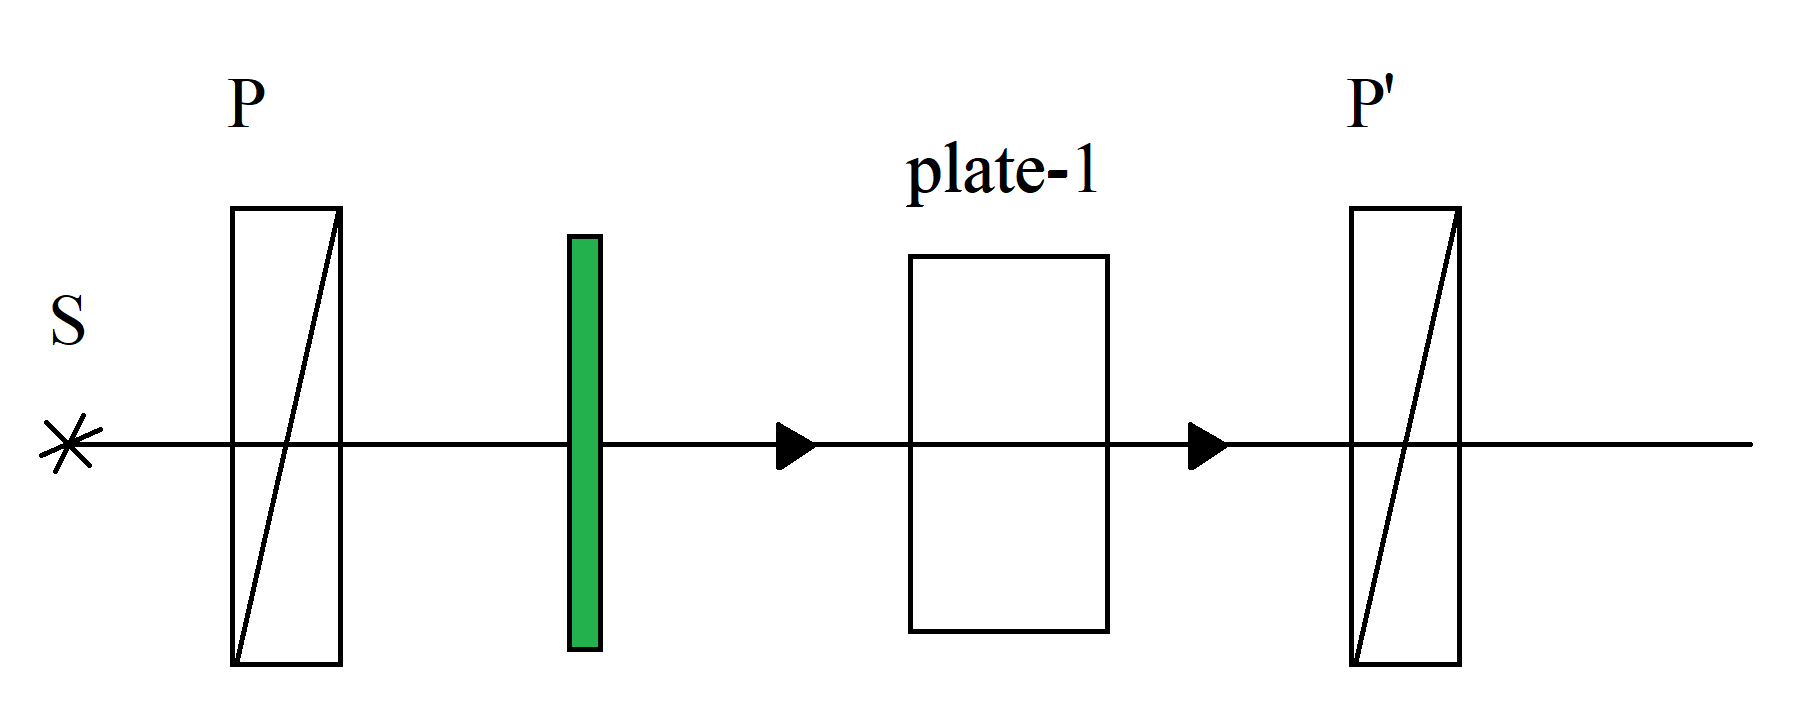
\includegraphics[width=1\textwidth]{images/greeeeeen.png}
    \caption{To the previous setup we add a green light-filter. And rotate the first polaraid so it is horizontal and the plate is  angled as $45^\circ$.}
    %\label{fig:}
\end{figure}
\end{minipage}
\hfill
\begin{minipage}{0.35\textwidth}
    By rotating the polaroid we obtain that plate-1 is $\lambda/4$, because it does not change the intensity, but it changes its polarization and creates phase difference $\pi/2$.
\end{minipage}
